\documentclass[11pt,letterpaper]{article}

%%%%%%%%%%%%%%%%%%%%%%%%%%%%%%%%%%%%%%%%%%%%%%%%%%%%%%%%%%%%%%%%%%%%%%%%%
\pagestyle{plain}                                                      %%
%%%%%%%%%% EXACT 1in MARGINS %%%%%%%                                   %%
\setlength{\textwidth}{6.5in}     %%                                   %%
\setlength{\oddsidemargin}{0in}   %% (It is recommended that you       %%
\setlength{\evensidemargin}{0in}  %%  not change these parameters,     %%
\setlength{\textheight}{8.5in}    %%  at the risk of having your       %%
\setlength{\topmargin}{0in}       %%  proposal dismissed on the basis  %%
\setlength{\headheight}{0in}      %%  of incorrect formatting!!!)      %%
\setlength{\headsep}{0in}         %%                                   %%
\setlength{\footskip}{.5in}       %%                                   %%
%%%%%%%%%%%%%%%%%%%%%%%%%%%%%%%%%%%%                                   %%
\newcommand{\required}[1]{\section*{\hfil #1\hfil}}                    %%
\renewcommand{\refname}{\hfil References Cited\hfil}                   %%
%\bibliographystyle{plain}                                              %%
%%%%%%%%%%%%%%%%%%%%%%%%%%%%%%%%%%%%%%%%%%%%%%%%%%%%%%%%%%%%%%%%%%%%%%%%%

%PUT YOUR MACROS HERE

\usepackage{amsmath}
\usepackage{amsfonts}
\usepackage{amssymb}
\usepackage{graphicx}
\usepackage{ulem}
\usepackage{placeins}

%\renewcommand{\thesection}{\Roman{section}} 
%\renewcommand{\thesubsection}{\thesection.\Roman{subsection}}

\title{NMR}

\date{}

\author{Ian Hunt-Isaak}


\begin{document}


\maketitle
\begin{abstract}
Using a TeachSpin Pulsed NMR PS1-D device we determined the spin relaxation constants $T_1$ and $T_2$ for a sample of mineral oil using standard techniques. The values were determined to be $T_1=21.69$ ms and $T_2=6.25$ ms. The theory and usage of NMR are discussed.
\end{abstract}
\section{Introduction}
\begin{enumerate}
\item NMR is for chemistry
\item allows to determine local magnetic field env
\end{enumerate}
\section{Background and Theory}

\begin{figure}[h!]
  \centering
      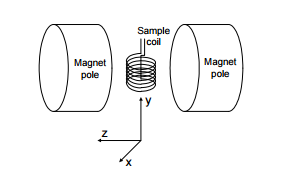
\includegraphics[scale=.4]{Sample_Env.png}
      \caption{The permanent magnetic field is directed along the $+z$ direction while the sample coil (pickup coil) detects magnetization of the sample in along the transverse ($y$) axis. Not shown are the RF coils used to tip the spins from alignment with the permanent field. Figure taken from A Conceptual Tour of NMR Ref. \cite{Concept_Tour}}
      \label{fig:Sample_Env}
\end{figure}
\subsection{T1}
\label{sub:T1_Theory}
The differential equation describing the Z axis magnetization under the influence of an external magnetic field applied along the axis is:
\begin{equation}
	\frac{dM_z}{dt}=\frac{M_0 - M_Z}{T_1}.
\end{equation}
Solving for $M_Z(t)$ results in:

\begin{equation}
\label{eq:T1_Fit}
	M_Z(t) = M_0-Ce^{\frac{-t}{T_1}},
\end{equation}
In the two pulse technique the first pulse, a $\pi$ pulse, sets the initial conditions allowing us to solve for $C$
\begin{align*}
	M_z(t=0)=-M_0,
\end{align*}

\begin{equation}
\label{eq:Mz}
	M_Z(t) = M_0(1-2e^{\frac{-t}{T_1}}),
\end{equation}
A $\frac{\pi}{2}$ pulse at time $\tau$ after the $\pi$ pulse allows us the measure $|M_Z(t)|$ so by varying the delay time $\tau$ we can collect data to fit with Eq. \ref{eq:T1_Fit} in order to determine $T_1$. However $M_Z$ is not always positive so the value $|M_Z(t)|$ which is measured cannot be fit immediately. 

Note that $M_Z$(t) is monotonically increasing so we know that we cannot directly measure $M_Z$, 
\subsection{T2}
Field inhomogeneities cause spins to precess at different rates leading to a loss of signal in the pickup coil due to the spins decohering. If this rate of decoherence, $T_2$*,  is short compared to the quantity $T_2$ a measurement of the FID will be a measurement of $T_2$* as the $T_2$ processes will not have had time to become significant. 


This issue can be avoided through a two-pulse technique known as spin echo, which forces the precessing spins to recohere allowing measurement of $T_2$. The application of a $\frac{\pi}{2}$ pulse tips the spins into the x-y plane where they begin to precess. Some time $\tau$ later the application of a $\pi$ pulse will reverse the direction of precession of the spins so that at $t=2\tau$ the spins will be coherent resulting in a peak in the signal detected. However this signal will be reduced compared to the amplitude of the FID resulting from the first pulse. The difference in amplitude of the first and second FID is the result of spins decaying via $T_2$ processes. 
From Ref. \cite{TeachspinManual} we have that spins tipped into the x-y plane by a $\frac{\pi}{2}$ pulse will decay to the Z axis with the following dependence:
\begin{equation}
M_{x,y}(t)=M_0e^{\frac{-t}{T_2}}
\end{equation}
At $t=0$ we have:
\begin{align}
M_{x,y}(t=0)=M_0
\end{align}
Resulting in:
\begin{equation}
\label{eq:T2_Fit}
\Delta V=M_0(1-e^{\frac{-t}{T_2}})
\end{equation}

\section{Experimental Procedures}
\begin{figure}[h!]
  \centering
      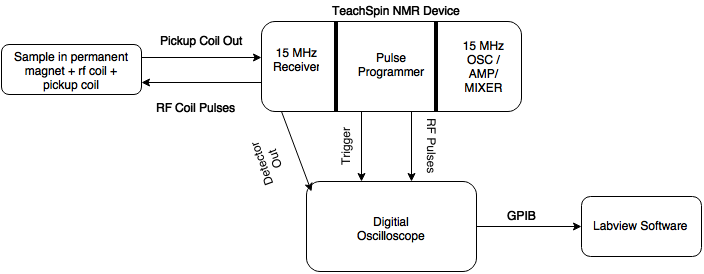
\includegraphics[scale=.4]{NMR_Block_Diagram.png}
      \caption{Block Diagram For the experiment. The TeachSpin device would provide RF pulses to flip the spins and output a clean signal to the oscilloscope from which measurement were made. For a diagram of the sample environment see Figure \ref{fig:Sample_Env}}
      \label{fig:Block_Diagram}
\end{figure}	

A TeachSpin Pulsed NMR PS1-D device was used to produce magnetic pulse and amplify the output of the pickup coil. The outputs were monitored with a Tektronix 200 MHz digital storage oscilloscope connected to a computer via labview. 

Prior to determination of the time constants $T_1$ and $T_2$ the frequency of the rf field was adjusted to the resonant frequency of the system. This was accomplished by minimizing the amplitude of the beat frequency signal of from the rf coil and the excitation applied.

The length of a $\frac{\pi}{2}$ pulse was determined by finding the minimum pulse width that resulted in a maximum of FID amplitude. After this the pulse width of a $\pi$ pulse was determined as the first pulse width value greater than the $\frac{\pi}{2}$ pulse width that caused no signal to be detected by the pickup coil.

\subsection{T1}
Following the theory developed in Section \ref{sub:T1_Theory} a $\pi$ pulse followed by a $\frac{\pi}{2}$ pulse was applied to the sample and the maximum voltage of the resulting peak was recorded along the delay time between peaks. As discussed above data points from the concave up portion of the data curve were taken as the negative values of M$_Z$.

This Voltage was fit to Eq. \ref{eq:T1_Fit} with a least squares method in order to determine $T_1$.
\subsection{T2}
\begin{enumerate}
\item how did
\end{enumerate}
\section{Results}
Data analysis was performed in Igor Pro the data was fit to functions via a least-squares method. Error was propagated using the Python Uncertainties package Ref. \cite{Uncertainties}.

\begin{figure}[h!]
  \centering
      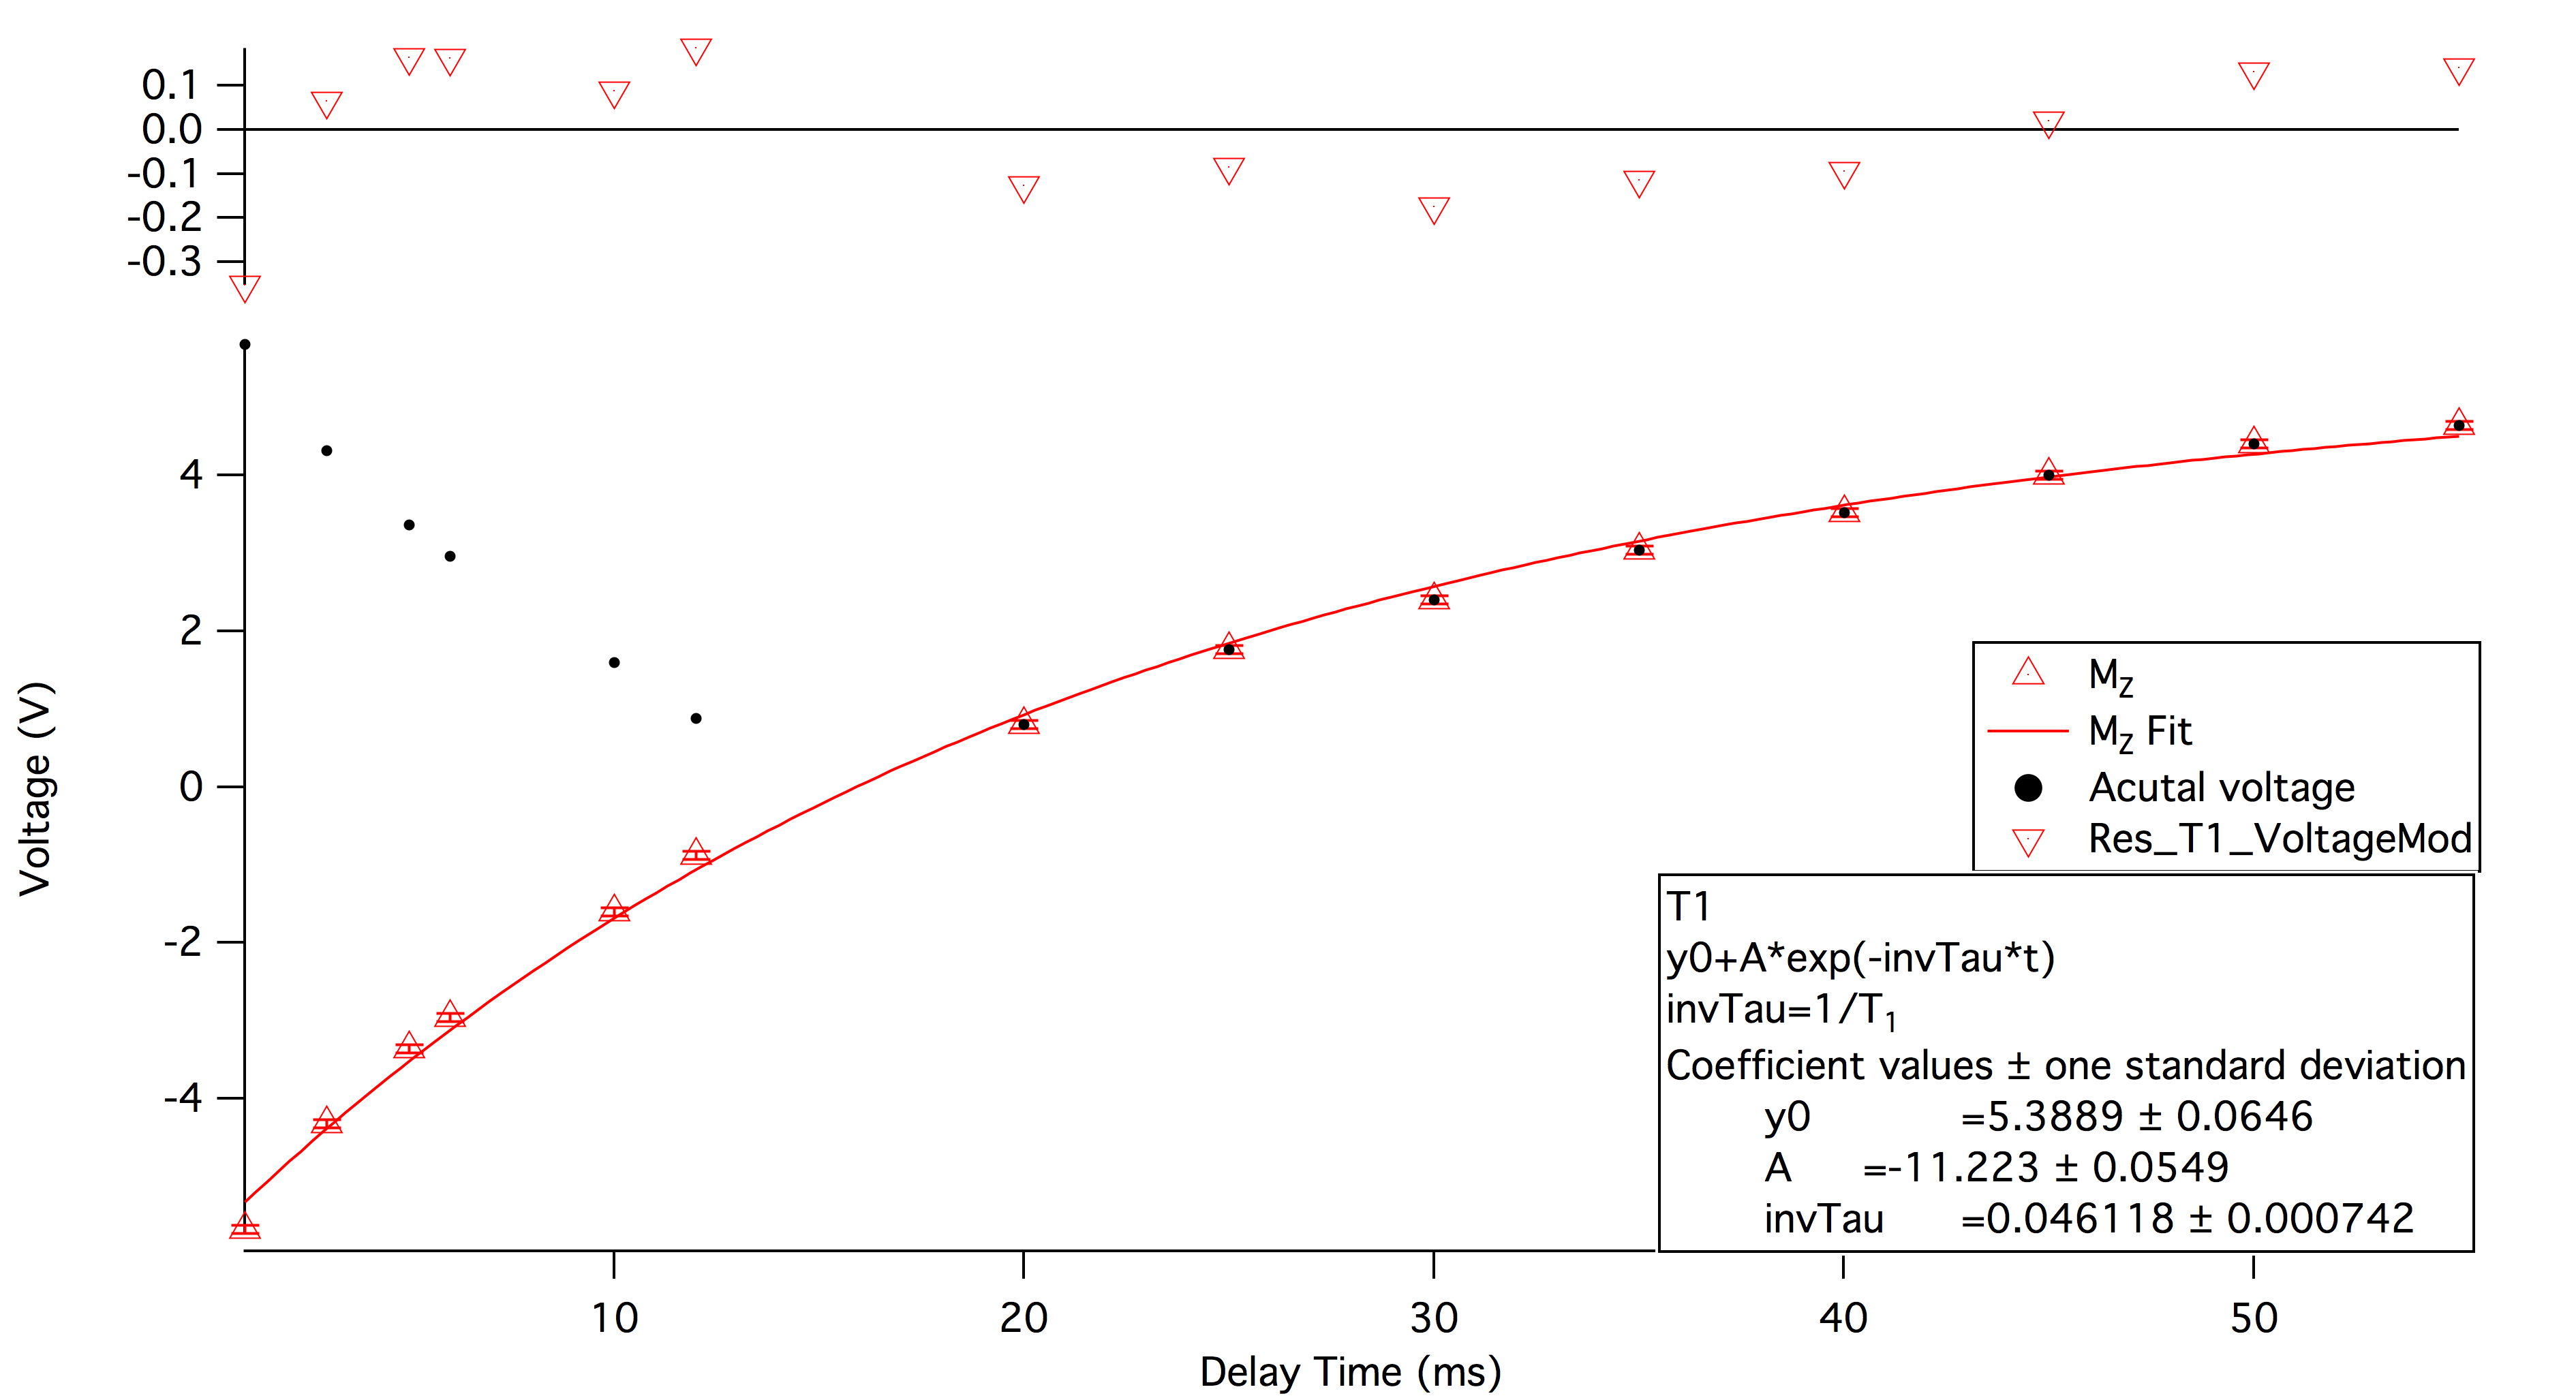
\includegraphics[scale=.3]{T1_Fit.png}
      \caption{{\small Determining $T_1$, Black dots are recorded $\Delta$V, red triangles are M$_Z$ as described in Theory Section}}
      \label{fig:T1_fit}
\end{figure}	

\begin{figure}
  \centering
      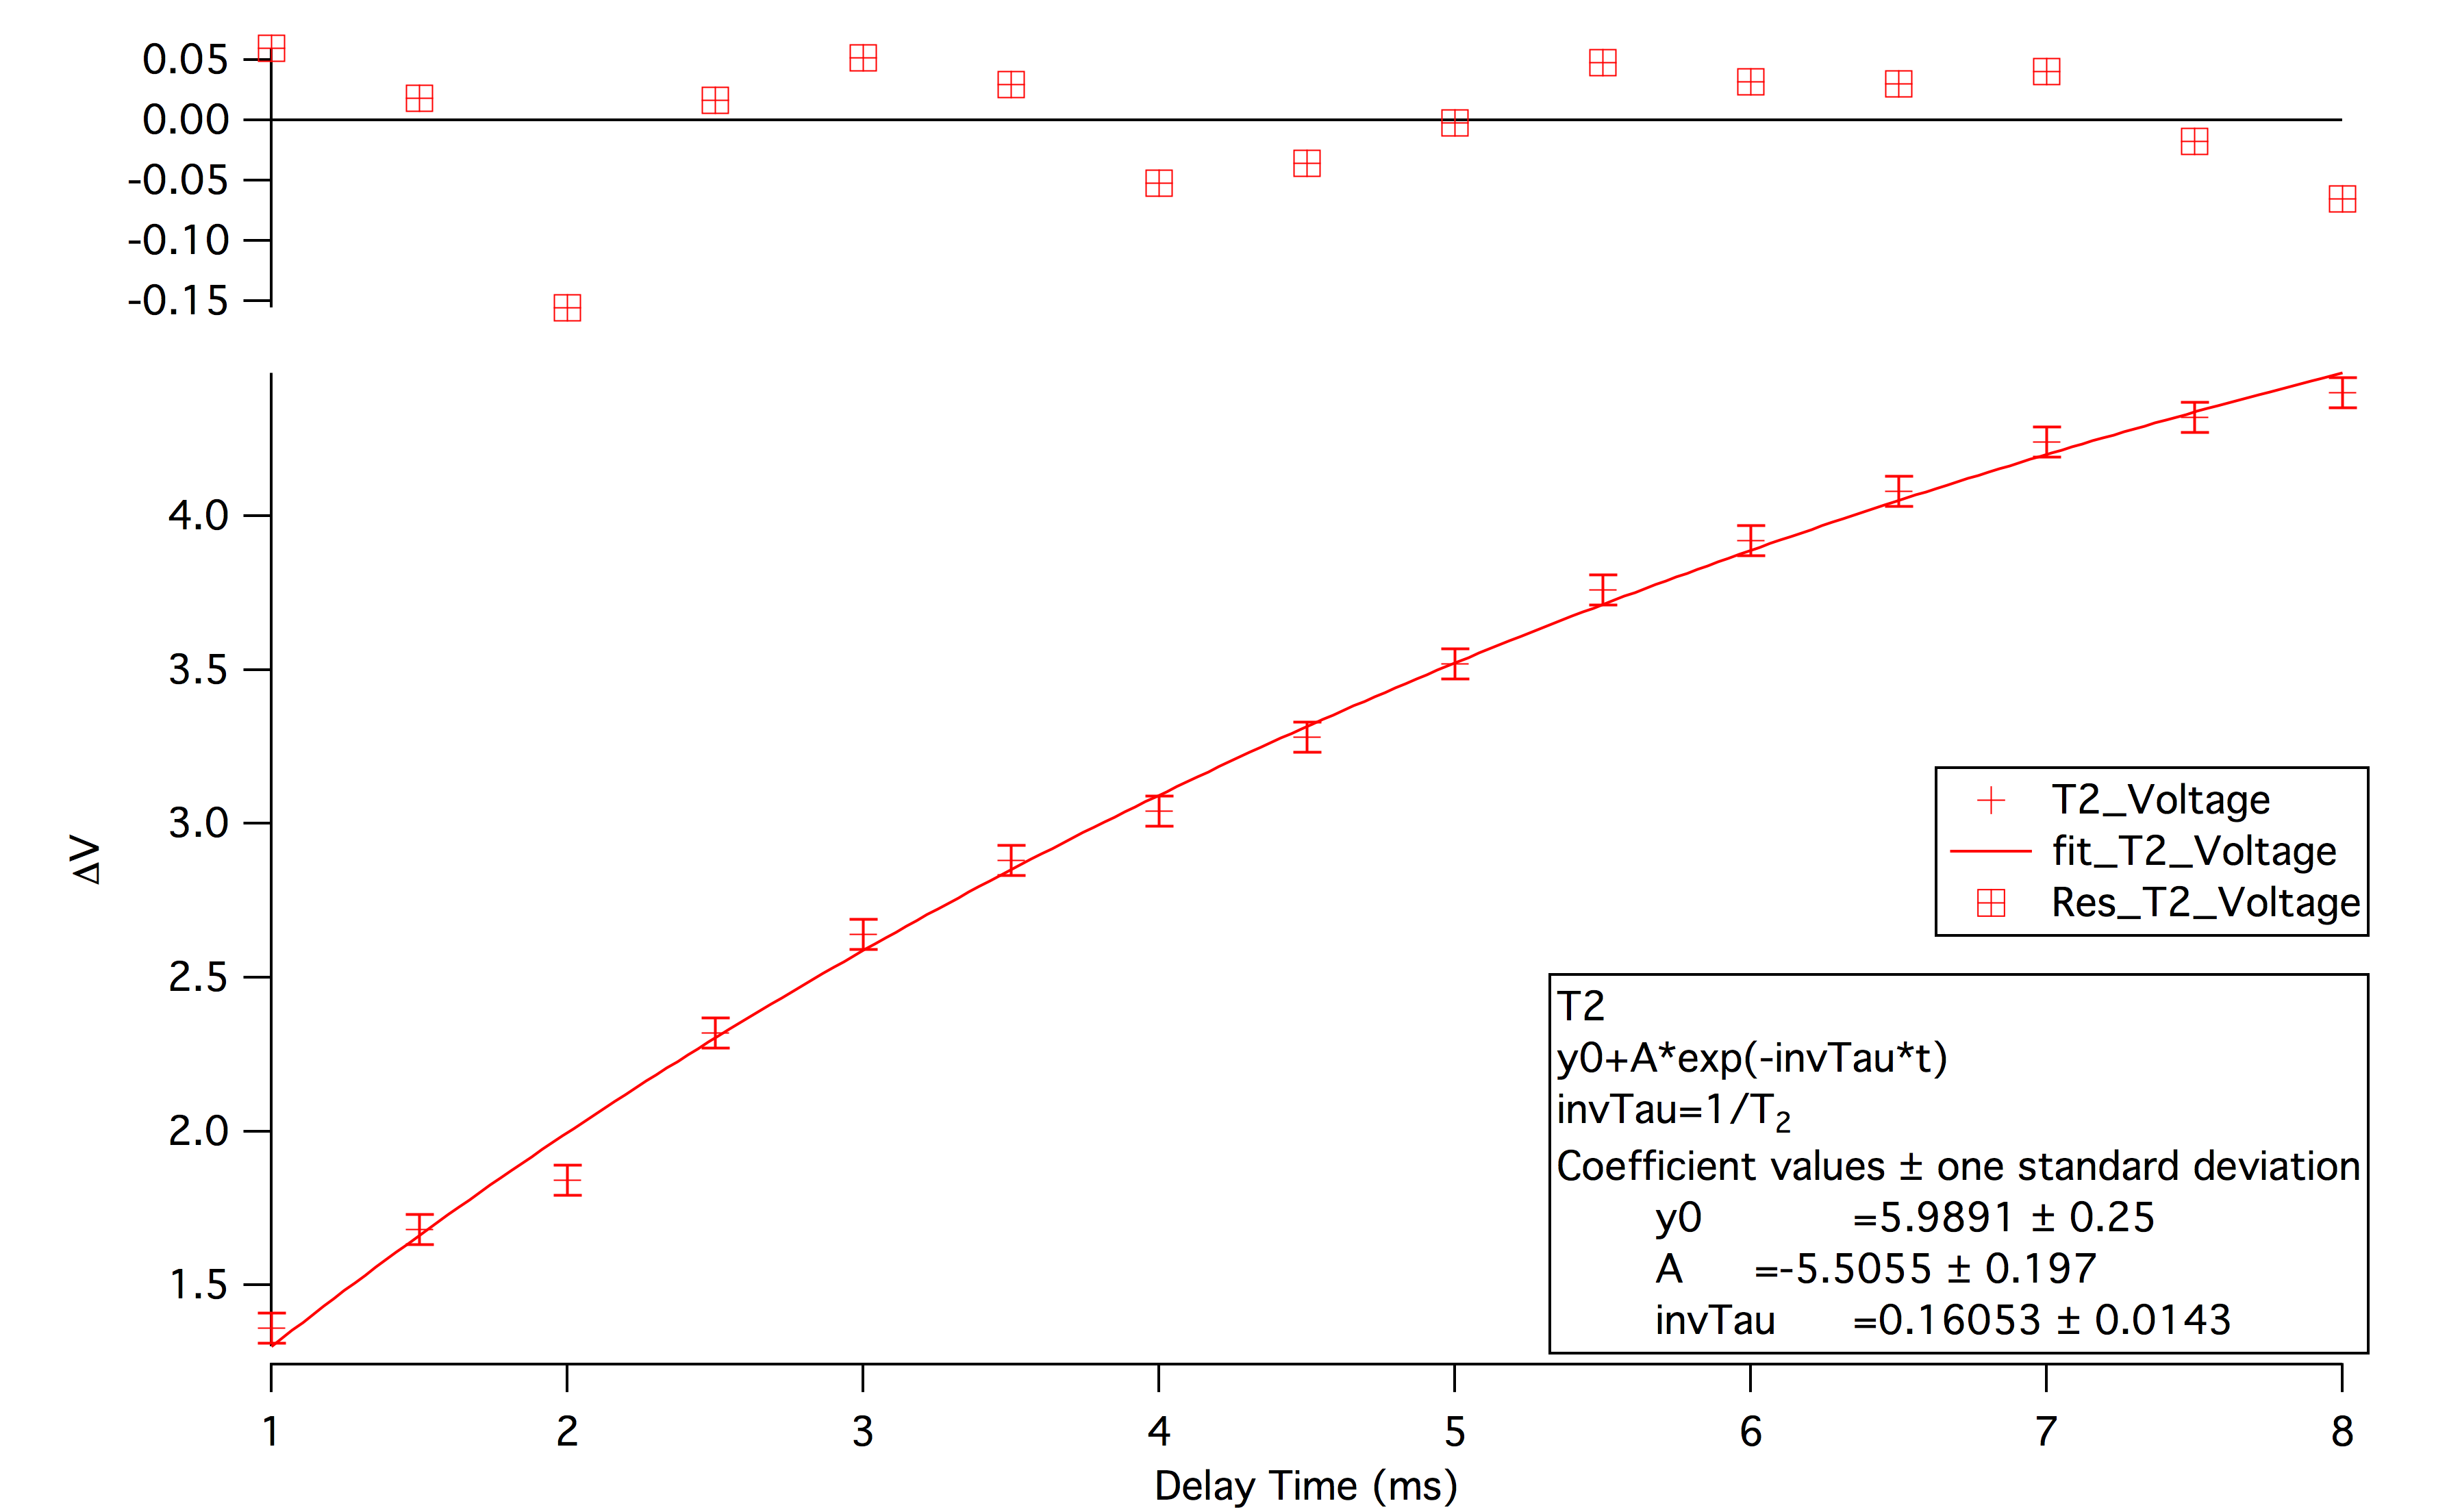
\includegraphics[scale=.3]{T2_Fit.png}
	\caption{Determining $T_2$}
\end{figure}
\FloatBarrier
Values the time constants were determined from these fits and are presented in Table \ref{Result_Table}

\begin{table}[!h]
\label{Result_Table}
\begin{center}
	\begin{tabular}{|c|c|c|}\hline
		Quantity & Value & Bianchini et. al \\ \hline\hline
		$T_2^*$ & .47 ms &  N/A \\ \hline
		$T_2$ & 6.23 $\pm$ .55 ms &  15.7 $\pm$ .01 ms \\ \hline
		$T_1$ & 21.68 $\pm$ .34 ms &  25.4 $\pm$ .07 ms\\ \hline
	
	\end{tabular}
		\caption{Values from this work and from Ref. \cite{Bianchini}}
			
		\end{center}
	\end{table}
As expected $T_2^*$ is significantly smaller than $T_2$. Also note that $T_1$ is $\sim$3x more than $T_2$. This is sensible as $T_1$ is associated with the realignment of the spins anti-aligned to the external field while $T_2$ corresponds to the realignment of spins which are perpendicular to the field. So $T_1$ corresponds to a much more dramatic realignment and also involves transfer of energy to the lattice.

Our values $T_1$ and $T_2$ are on the same order of magnitude as as those found by Bianchini and Coffey, that they are several standard deviations apart is not significant as Mineral Oil is not a standard substance. We note that our uncertainties are much larger than those found by Bianchini and Coffey

\subsection{Uncertainty Budget}
\begin{table}[!h]
	\begin{center}
		\begin{tabular}{|c|c|c|c|} \hline 
			Source & Quantity&  Error in Quantity  & Propagated Error  \\ \hline \hline
			Statistical Error & $T_1$ & .35 (ms) & .35 (ms)\\ \hline 
			Statistical Error & $T_2$ & .6 (ms)& .6 (ms)\\ \hline
			Pulse Width& $\tau$ & 5\% & Negligible\\
			\hline
		\end{tabular}
	\end{center}
\end{table}
Due to the use of oscilloscope cursors to determine the voltages for determining $T_1$ and $T_2$ we estimate the error in the voltage values as $\pm .05$V. This combined with statistical errors in fitting is the dominant source of uncertainty. However as noted in Section \ref{sec:ChiSq} the error on the voltage may have been underestimated.

The other source of the uncertainty was the the inability of to produce an exact $\frac{\pi}{2}$ pulse. However this is ultimately a negligible effect as the probability of excitation is described by a sin curve and a $\frac{\pi}{2}$ pulse is located at an anti-node of this curve and so a small deviation in pulse width will not have a dramatic effect.

I would like to try to calculate $T_1$ and $T_2$ with a few pulse widths in order to get a better sense of the error that this introduces.
\subsection{$\chi^2$ analysis}
\label{sec:ChiSq}
Igor produces $\chi^2$ values when performing a least squares fit, $\tilde{\chi}^2$ values were determined using:
\begin{align}
\tilde{\chi}^2=\frac{\chi^2}{d}
\\
d=N-c
\end{align}
Where c is the number of constraints, three for the equations fit to, and N is number of points.
\begin{table}[!h]
	\begin{center}
		\begin{tabular}{|c|c|c|c|c|} \hline 
			Quantity & $\chi^2$&Deg Freedom&$\tilde{\chi}^2$  &  Probability \\ \hline \hline
			$T_1$ & 133.9 & 11 & 12.17 &  $\approx0$ \%   \\ \hline 
			$T_2$ & 18.55 & 12 & 1.54 & 12 \%   \\ \hline
		\end{tabular} \\
		Probabilities were determined from Ref. \cite{TaylorError}
	\end{center}
\end{table}

From the residuals of the fits we can see that our fits are not bad. However our $\chi^2$ analysis would seem to indicate a flawed model. A possible reconciliation of this is that we underestimated our uncertainty or did not account for a systematic error. Though the latter seems unlikely due to our residuals.

\section{Conclusions}
\section{Acknowledgements}
Pete Sinn was invaluable as a Lab Partner when performing this experiment.

\begin{thebibliography}{99}
\bibitem{Concept_Tour} Barbara Wolff-Reichert, Conceptual Tour of PNMR, 2008 
\bibitem{TeachspinManual} Teachspin Instructional Pulsed NMR Apparatus Manual, Department of Physics and Astronomy, Knoxville, TN
\bibitem{TaylorError} J.R. Taylor, {\it Introduction to Error Analysis}, (University Science Books, Sausalito, 1997)
\bibitem{Bianchini} L. Bianchini, L. Coffey, Physics Department, Brandeis University, NMR Techniques Applied to Mineral Oil, Water, and Ethanol (2010)
\bibitem{Uncertainties} {\it Uncertainties}: a Python package for calculations with uncertainties, Eric O. LEBIGOT, http://pythonhosted.org/uncertainties/

\end{thebibliography}
\end{document}